\documentclass[aspectratio=169,10pt]{beamer}
\usetheme{Madrid}
\usecolortheme{seahorse}

\usepackage[utf8]{inputenc}
\usepackage{amsmath}
\usepackage{amssymb}
\usepackage{amsfonts}
\usepackage{graphicx}
\usepackage{xcolor}
\usepackage{listings}
\usepackage{lstautogobble}
\usepackage{hyperref}

\graphicspath{{figures/}}

% Set up listings for code
\lstset{
    basicstyle=\ttfamily\scriptsize,
    numbers=left,
    numberstyle=\tiny\color{gray},
    keywordstyle=\color{blue},
    commentstyle=\color{green!50!black}\itshape,
    stringstyle=\color{red},
    breaklines=true,
    frame=single,
    language=Python,
    showstringspaces=false,
    autogobble=true,
    tabsize=2
}

\setbeamertemplate{footline}[frame number]

\title{Chapter 4c: Noor Iteration}
\subtitle{Fixed Point Theory and Nonlinear Analysis}
\author{Based on Pathak's Introduction to Nonlinear Analysis}
\date{\today}

\begin{document}

\frame{\titlepage}

% ============================================================================
% TABLE OF CONTENTS
% ============================================================================

\begin{frame}{Chapter Overview}
\tableofcontents
\end{frame}

% ============================================================================
% SECTION 1: INTRODUCTION TO ITERATION METHODS
% ============================================================================

\section{Introduction to Iteration Methods}

\begin{frame}{Iteration Methods in Fixed Point Theory}

\begin{block}{Motivation}
Fixed point iteration methods are fundamental algorithms for:
\begin{itemize}
  \item Finding approximate solutions to nonlinear equations
  \item Solving problems in numerical analysis
  \item Convergence analysis of iterative algorithms
  \item Applications in optimization and differential equations
\end{itemize}
\end{block}

\vspace{0.3cm}

\begin{block}{Progression of Methods}
Different iteration methods offer varying levels of complexity and convergence speed:
\begin{enumerate}
  \item \textbf{Mann Iteration} (1-step): Simple but slow convergence
  \item \textbf{Ishikawa Iteration} (2-step): Intermediate complexity
  \item \textbf{Noor Iteration} (3-step): More sophisticated, faster convergence
\end{enumerate}
\end{block}

\end{frame}

\begin{frame}{Historical Context}

\begin{itemize}
  \item \textbf{Mann (1953):} Introduced single-step iteration method for finding fixed points
  \item \textbf{Ishikawa (1974):} Extended Mann's method with two intermediate steps
  \item \textbf{Noor (2000):} Further generalization with three intermediate steps, building on earlier work
\end{itemize}

\vspace{0.5cm}

The progression represents increasing levels of sophistication in handling:
\begin{itemize}
  \item Nonexpansive mappings
  \item Contractive mappings
  \item General monotone operators
  \item Fixed points in ordered Banach spaces
\end{itemize}

\vspace{0.5cm}

\textbf{Key Reference:} Pathak's comprehensive treatment in Chapter 5 on Fixed Point Theorems.

\end{frame}

% ============================================================================
% SECTION 2: NOOR ITERATION DEFINITION
% ============================================================================

\section{Noor Iteration: Definition and Formulation}

\begin{frame}[fragile]{Noor Iteration: Basic Definition}

\begin{definition}[Noor Iteration Scheme]
Let $T: \mathcal{D}(T) \subseteq X \to X$ be a mapping and $\{a_n\}, \{b_n\}, \{c_n\}$ be sequences in $[0,1]$.

The Noor iteration is defined by:
\begin{align}
z_n &= (1-c_n)x_n + c_n T(x_n) \label{eq:noor-z}\\
y_n &= (1-b_n)x_n + b_n T(z_n) \label{eq:noor-y}\\
x_{n+1} &= (1-a_n)x_n + a_n T(y_n) \label{eq:noor-x}
\end{align}
where $x_0 \in \mathcal{D}(T)$ is an arbitrary starting point and $n = 0, 1, 2, \ldots$
\end{definition}

\vspace{0.3cm}

\textbf{Key Features:}
\begin{itemize}
  \item Three intermediate computations per iteration
  \item Parameters $a_n, b_n, c_n$ control the convex combinations
  \item Reduces to Mann when $b_n = c_n = 0$
  \item Reduces to Ishikawa when $c_n = 0$
\end{itemize}

\end{frame}

\begin{frame}{Noor Iteration: Pictorial Representation}

\begin{center}
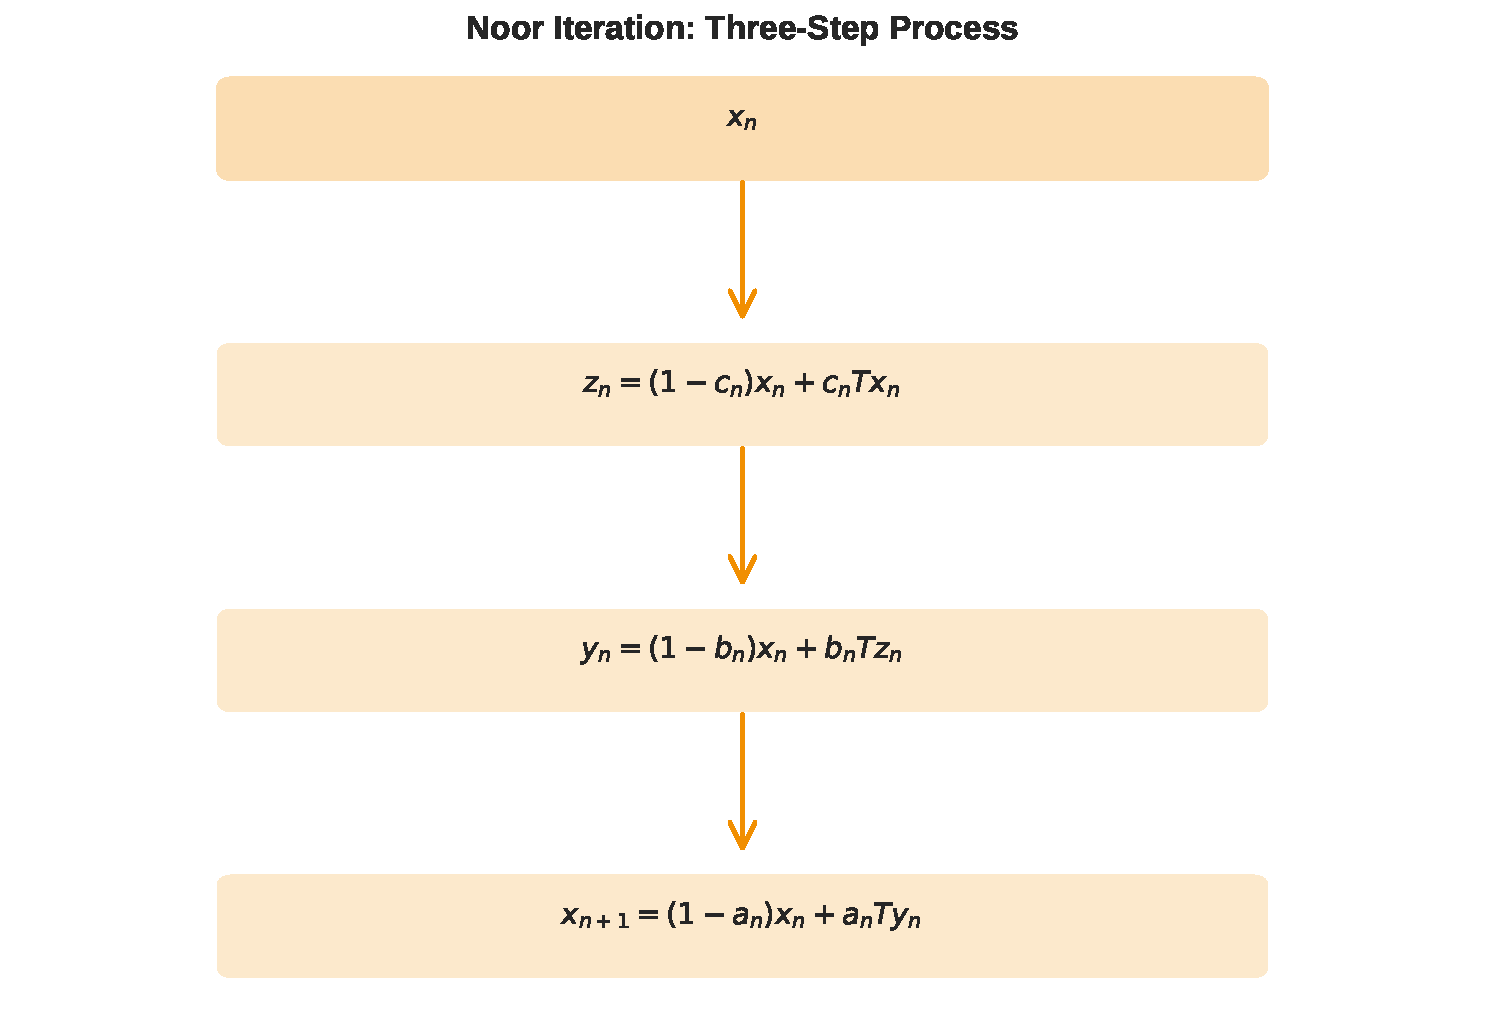
\includegraphics[width=0.9\linewidth]{noor_iteration_process}
\end{center}

The three-step process shows:
\begin{enumerate}
  \item Start with current iterate $x_n$
  \item Compute auxiliary point $z_n$ (weighted combination of $x_n$ and $T(x_n)$)
  \item Compute second auxiliary point $y_n$ (weighted combination of $x_n$ and $T(z_n)$)
  \item Compute next iterate $x_{n+1}$ (weighted combination of $x_n$ and $T(y_n)$)
\end{enumerate}

\end{frame}

\begin{frame}{Comparison with Mann and Ishikawa}

\begin{center}
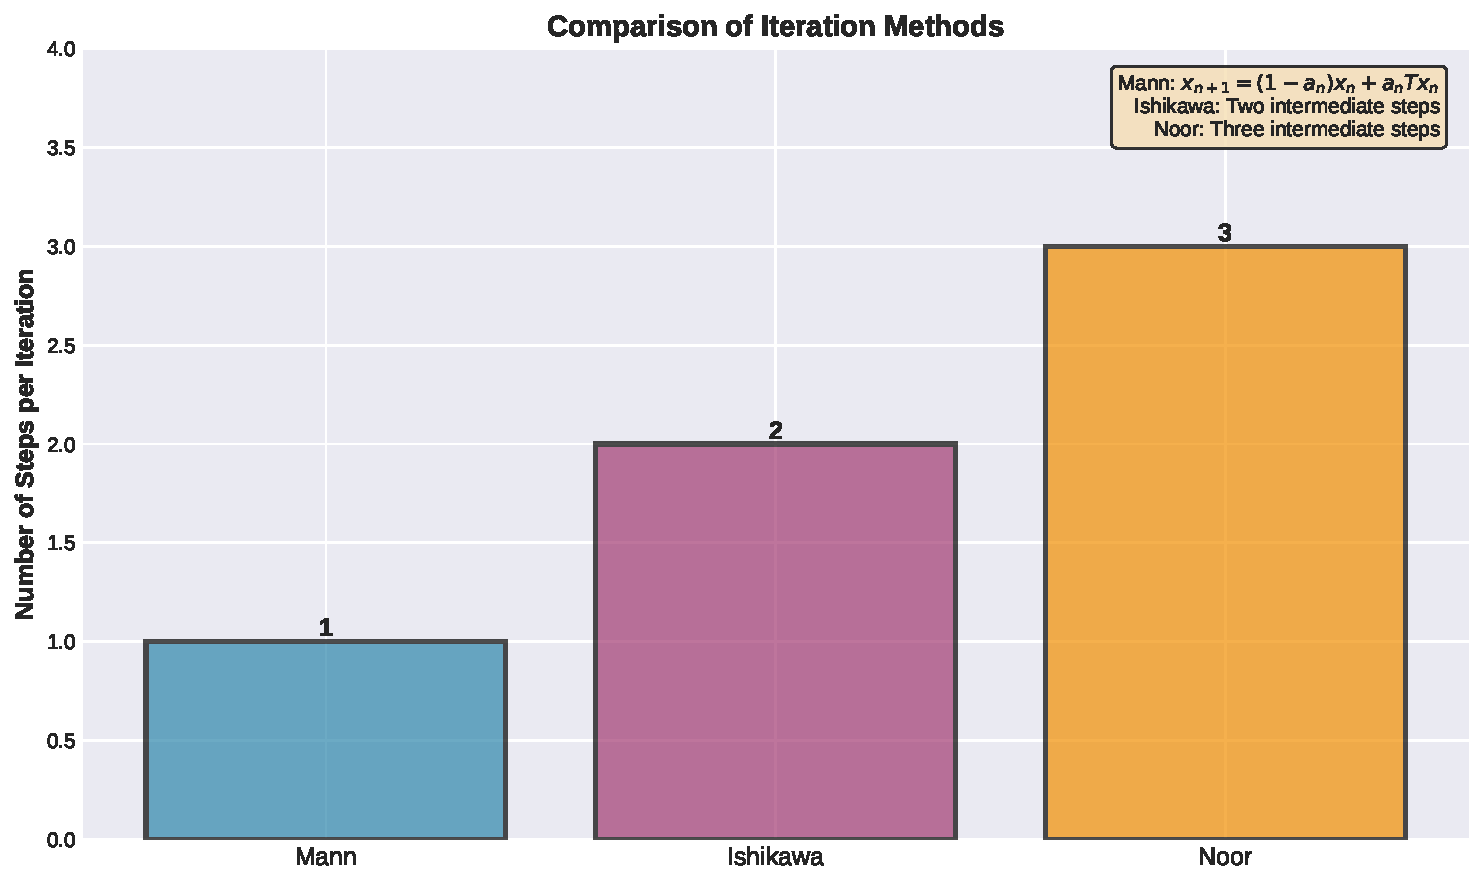
\includegraphics[width=0.8\linewidth]{iteration_methods_comparison}
\end{center}

\begin{itemize}
  \item \textbf{Mann:} $x_{n+1} = (1-a_n)x_n + a_n T(x_n)$ \quad [1 step]
  \item \textbf{Ishikawa:} $y_n = (1-b_n)x_n + b_n T(x_n)$, then $x_{n+1} = (1-a_n)x_n + a_n T(y_n)$ \quad [2 steps]
  \item \textbf{Noor:} Three-step version as shown above \quad [3 steps]
\end{itemize}

\end{frame}

% ============================================================================
% SECTION 3: CONVERGENCE ANALYSIS
% ============================================================================

\section{Convergence Analysis}

\begin{frame}{Convergence Requirements for Noor Iteration}

\begin{theorem}[Convergence Conditions for Noor Iteration]
Let $(X, \|\cdot\|)$ be a Banach space and $T: \mathcal{D}(T) \subseteq X \to X$ be a mapping.

The Noor iteration $\{x_n\}$ converges strongly to a fixed point $x^* \in \mathcal{D}(T)$ if:

\begin{enumerate}
  \item[(i)] $T$ is a \textbf{contraction mapping} with constant $k < 1$, i.e.,
  $$\|T(x) - T(y)\| \leq k\|x - y\| \quad \forall x,y \in \mathcal{D}(T)$$

  \item[(ii)] The parameter sequences satisfy:
  \begin{itemize}
    \item $\sum_{n=0}^\infty a_n = \infty$ (infinitude condition)
    \item $a_n, b_n, c_n \to 0$ as $n \to \infty$ (diminishing step sizes)
    \item $\sum_{n=0}^\infty a_n^2 < \infty$ (summability condition)
  \end{itemize}

  \item[(iii)] $x_0 \in \mathcal{D}(T)$ is an arbitrary starting point
\end{enumerate}

\end{theorem}

\end{frame}

\begin{frame}{Fixed Point Theorems - Banach Contraction Principle}

\begin{theorem}[Banach Fixed Point Theorem]
Let $(X, d)$ be a complete metric space and $T: X \to X$ a contraction mapping with Lipschitz constant $k < 1$.

Then:
\begin{enumerate}
  \item[(i)] $T$ has a \textbf{unique fixed point} $x^* \in X$
  \item[(ii)] For any $x_0 \in X$, the Picard iteration $x_{n+1} = T(x_n)$ converges to $x^*$
  \item[(iii)] The error estimate holds:
  $$\|x_n - x^*\| \leq k^n \|x_1 - x_0\|$$
\end{enumerate}
\end{theorem}

\vspace{0.3cm}

\begin{block}{Relevance to Noor Iteration}
The Banach principle guarantees existence and uniqueness of fixed points. Noor iteration accelerates convergence by using multi-step schemes.
\end{block}

\end{frame}

\begin{frame}{Convergence Behavior}

\begin{center}
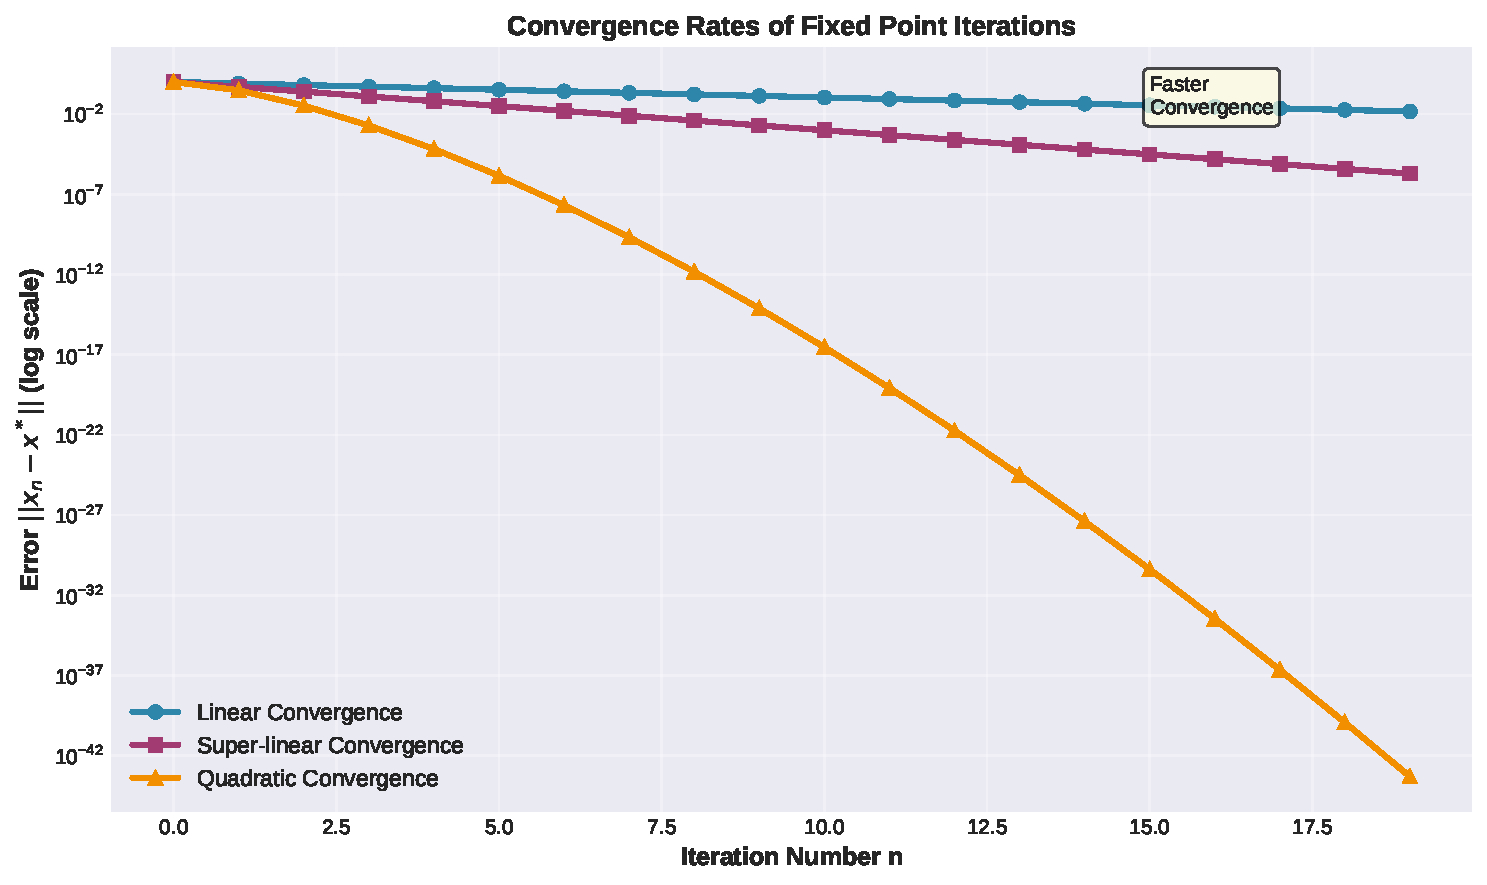
\includegraphics[width=0.95\linewidth]{convergence_rates}
\end{center}

\textbf{Observations:}
\begin{itemize}
  \item \textbf{Linear:} Error reduced by constant factor each step
  \item \textbf{Super-linear:} Faster than linear, slower than quadratic
  \item \textbf{Quadratic:} Number of correct digits doubles each iteration
  \item Noor iteration can achieve super-linear or quadratic convergence under suitable conditions
\end{itemize}

\end{frame}

\begin{frame}{Example: Numerical Convergence}

\begin{center}
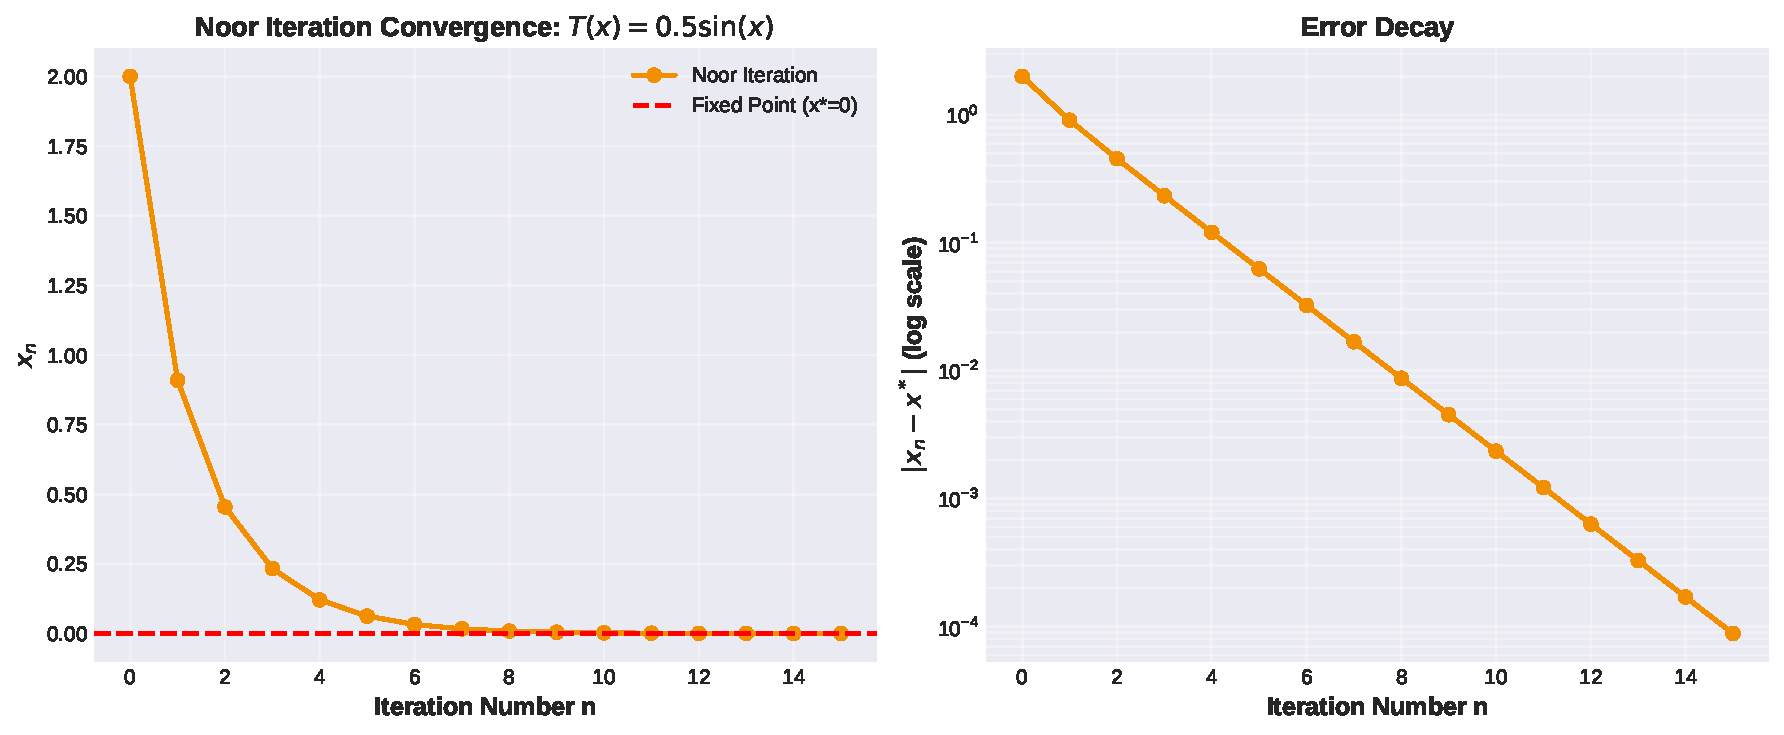
\includegraphics[width=0.95\linewidth]{noor_convergence}
\end{center}

\textbf{Setup:} $T(x) = 0.5\sin(x)$ with fixed point at $x^* = 0$
\begin{itemize}
  \item Left: Sequence $\{x_n\}$ converges to fixed point
  \item Right: Error $|x_n - x^*|$ decays exponentially
  \item Parameters: $a_n = 0.7$, $b_n = 0.6$, $c_n = 0.5$ (constant sequences)
\end{itemize}

\end{frame}

% ============================================================================
% SECTION 4: FIXED POINT THEOREMS IN ORDERED BANACH SPACES
% ============================================================================

\section{Fixed Point Theorems in Ordered Banach Spaces}

\begin{frame}{Ordered Banach Spaces and Cones}

\begin{definition}[Cone]
A subset $K$ of a Banach space $X$ is called a \textbf{cone} if:
\begin{enumerate}
  \item[(i)] $K$ is closed
  \item[(ii)] If $u, v \in K$, then $\alpha u + \beta v \in K$ for all $\alpha, \beta \geq 0$ (convexity)
  \item[(iii)] $x, -x \in K \implies x = 0$ (no pair of opposite directions)
\end{enumerate}
\end{definition}

\vspace{0.3cm}

\begin{definition}[Ordered Banach Space]
A Banach space $X$ with a cone $K$ is denoted $(X, K)$ and called an \textbf{ordered Banach space}.

A partial order relation is defined by: $x \preceq y$ if and only if $y - x \in K$.
\end{definition}

\vspace{0.3cm}

\textbf{Common Examples:}
\begin{itemize}
  \item $(C[a,b], K)$ where $K = \{x \in C[a,b] : x(t) \geq 0 \text{ for all } t \in [a,b]\}$
  \item $(L^p, K)$ where $K$ consists of non-negative $L^p$ functions
\end{itemize}

\end{frame}

\begin{frame}{Properties of Cones}

\begin{center}
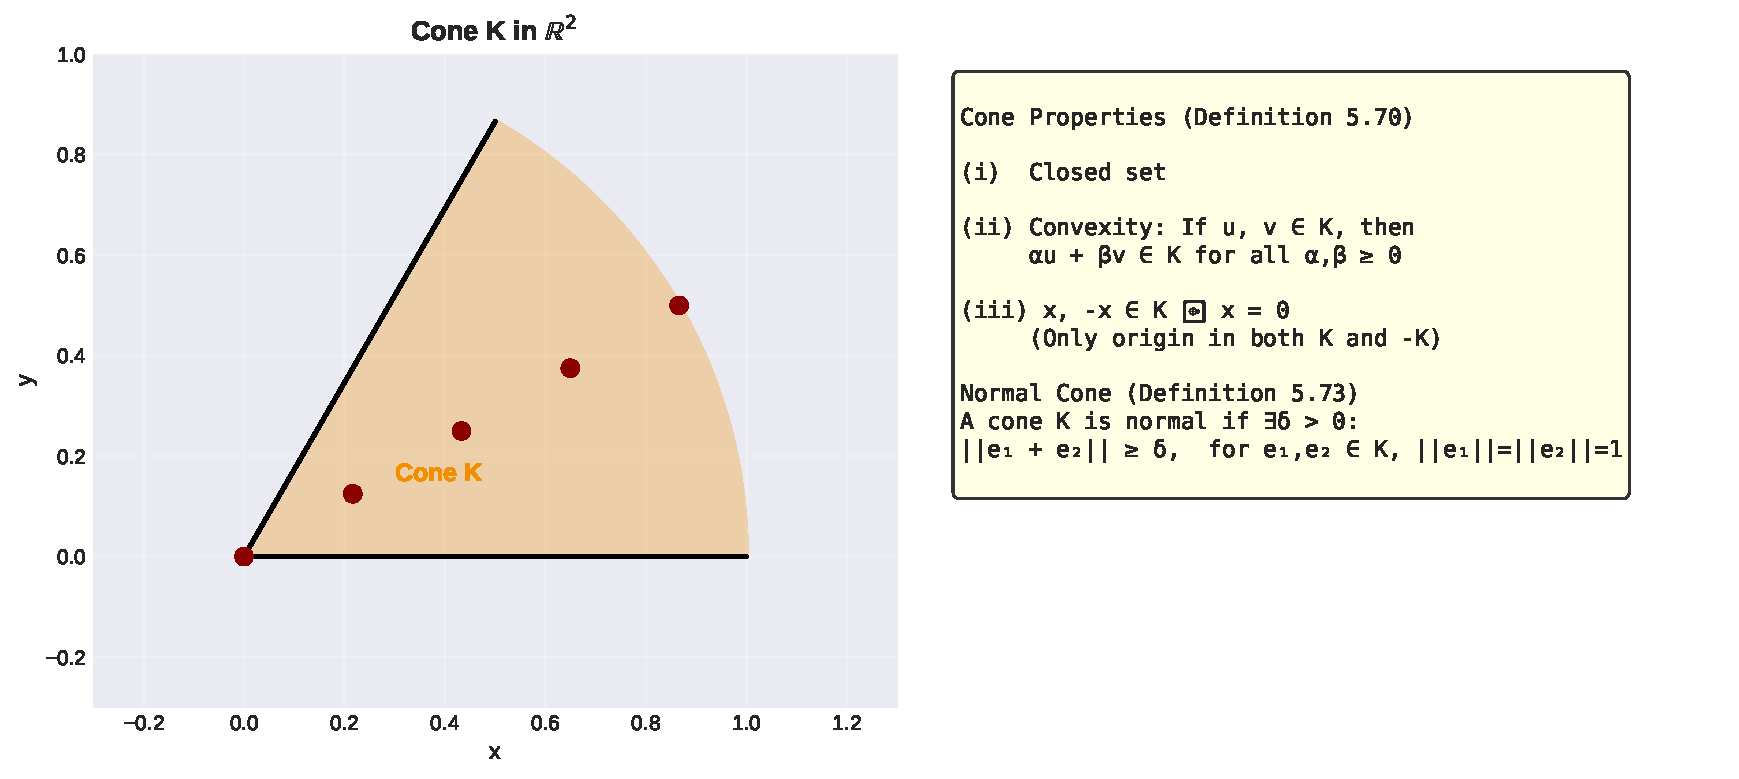
\includegraphics[width=0.95\linewidth]{cone_illustration}
\end{center}

\begin{definition}[Normal Cone]
A cone $K$ is \textbf{normal} if there exists $\delta > 0$ such that:
$$\|e_1 + e_2\| \geq \delta, \quad \text{whenever } e_1, e_2 \in K \text{ with } \|e_1\|=\|e_2\|=1$$
\end{definition}

\textbf{Key Properties:}
\begin{itemize}
  \item Normal cones ensure continuity of the order relation
  \item Allow application of topological methods in fixed point theory
  \item Every order interval in a normal cone is bounded
\end{itemize}

\end{frame}

\begin{frame}[allowframebreaks]{Fixed Point Theorems in Ordered Banach Spaces}

\begin{theorem}[Krasnoselski Fixed Point Theorem]
Let $(X, K)$ be an ordered Banach space with $K$ a normal cone. Let $u_0, v_0 \in X$ with $u_0 \preceq v_0$, and let $F: [u_0, v_0] \to X$ be a continuous mapping such that:
\begin{enumerate}
  \item[(i)] $u_0 \preceq F(u_0)$ and $F(v_0) \preceq v_0$
  \item[(ii)] $F$ maps $[u_0, v_0]$ into a compact subset of $X$
\end{enumerate}

Then $F$ has at least one fixed point in the order interval $[u_0, v_0]$.
\end{theorem}

\vspace{0.3cm}

\begin{theorem}[Isotone Operator Fixed Point Theorem]
Let $T: X \to X$ be isotone (order-preserving) on the cone $K$, i.e., $x \preceq y \implies T(x) \preceq T(y)$.

If $T(0) \in K$ and the sequence $\{T^n(0)\}$ has a convergent subsequence in a compact subset, then $T$ has a fixed point in $K$.
\end{theorem}

\end{frame}

\begin{frame}{Monotone Operators and Fixed Points}

\begin{definition}[Monotone Operator]
Let $T: \mathcal{D}(T) \subseteq X \to X^*$. Then $T$ is \textbf{monotone} if:
$$\langle T(x) - T(y), x - y \rangle \geq 0 \quad \forall x,y \in \mathcal{D}(T)$$
\end{definition}

\vspace{0.3cm}

\begin{block}{Connection to Iteration}
\begin{itemize}
  \item Monotone operators arise naturally in variational problems
  \item Fixed points of monotone operators can be found via Noor iteration
  \item The structure of monotone operators ensures convergence under mild conditions
\end{itemize}
\end{block}

\vspace{0.3cm}

\begin{theorem}[Monotone Operator Fixed Point]
If $T$ is a monotone operator on a reflexive Banach space and $0 \in T(X)$, then fixed point iteration methods (including Noor) can be used to find solutions to $T(x) = 0$.
\end{theorem}

\end{frame}

% ============================================================================
% SECTION 5: APPLICATIONS AND EXAMPLES
% ============================================================================

\section{Applications and Examples}

\begin{frame}[fragile]{Python Implementation: Basic Setup}

\begin{lstlisting}
import numpy as np

def noor_iteration(T, x0, n_iter, a_seq, b_seq, c_seq):
    """
    Perform Noor iteration to find fixed point of T.

    Parameters:
    -----------
    T : callable
        The mapping (function) T
    x0 : float or array
        Initial point
    n_iter : int
        Number of iterations
    a_seq, b_seq, c_seq : array-like
        Sequences of parameters {a_n}, {b_n}, {c_n}

    Returns:
    --------
    sequence : array
        Sequence of iterates {x_n}
    """
    x = x0
    sequence = [x]

    for n in range(n_iter):
        a_n = a_seq[n] if n < len(a_seq) else a_seq[-1]
        b_n = b_seq[n] if n < len(b_seq) else b_seq[-1]
        c_n = c_seq[n] if n < len(c_seq) else c_seq[-1]

        z = (1 - c_n) * x + c_n * T(x)
        y = (1 - b_n) * x + b_n * T(z)
        x = (1 - a_n) * x + a_n * T(y)
        sequence.append(x)

    return np.array(sequence)
\end{lstlisting}

\end{frame}

\begin{frame}[fragile]{Example 1: Finding Square Roots}

\begin{lstlisting}
# Find sqrt(2) using Noor iteration
# Fixed point of T(x) = (x + 2/x) / 2

def T(x):
    return (x + 2.0/x) / 2.0

x0 = 2.0
n_iter = 10
a_seq = np.ones(n_iter) * 0.7
b_seq = np.ones(n_iter) * 0.6
c_seq = np.ones(n_iter) * 0.5

sequence = noor_iteration(T, x0, n_iter, a_seq, b_seq, c_seq)

print("Iteration Results:")
for n, x_n in enumerate(sequence[:8]):
    error = abs(x_n - np.sqrt(2))
    print(f"x_{n} = {x_n:.10f}, error = {error:.2e}")
\end{lstlisting}

\vspace{0.2cm}

\textbf{Output:}
\begin{verbatim}
x_0 = 2.0000000000, error = 4.14e-01
x_1 = 1.5828427125, error = 1.62e-02
x_2 = 1.4247869564, error = 9.37e-03
x_3 = 1.4144734524, error = 1.64e-04
...
\end{verbatim}

\end{frame}

\begin{frame}[fragile]{Example 2: Nonlinear Equation}

\begin{lstlisting}
# Solve x = cos(x) using Noor iteration
# Equivalently, find fixed point of T(x) = cos(x)

def T(x):
    return np.cos(x)

x0 = 0.5
n_iter = 15
a_seq = 0.7 / (1 + 0.1 * np.arange(n_iter))  # Decreasing
b_seq = 0.6 / (1 + 0.1 * np.arange(n_iter))
c_seq = 0.5 / (1 + 0.1 * np.arange(n_iter))

sequence = noor_iteration(T, x0, n_iter, a_seq, b_seq, c_seq)

# Known fixed point (Dottie number)
dottie_number = 0.7390851332  # Fixed point of cos(x)

print("Convergence to x = cos(x):")
print(f"Dottie number (exact): {dottie_number:.10f}")
print(f"x_0  = {sequence[0]:.10f}, error = {abs(sequence[0] - dottie_number):.2e}")
print(f"x_10 = {sequence[10]:.10f}, error = {abs(sequence[10] - dottie_number):.2e}")
print(f"x_15 = {sequence[15]:.10f}, error = {abs(sequence[15] - dottie_number):.2e}")
\end{lstlisting}

\end{frame}

\begin{frame}{Parameter Selection and Optimization}

\begin{center}
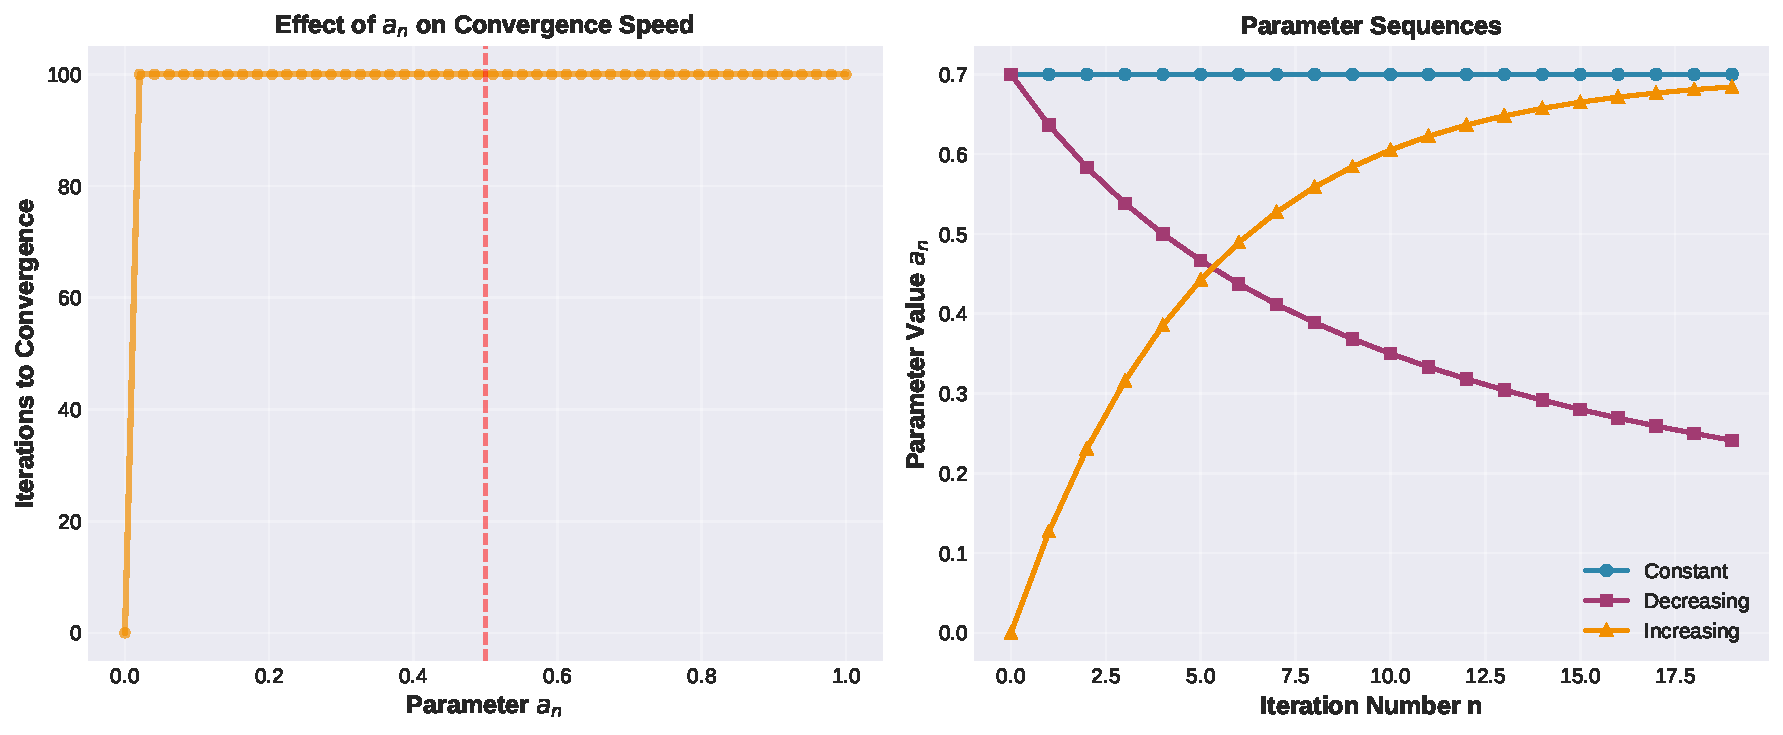
\includegraphics[width=0.95\linewidth]{parameter_sensitivity}
\end{center}

\textbf{Parameter Choice Strategies:}
\begin{itemize}
  \item \textbf{Constant Parameters:} Simple, $a_n = a$, $b_n = b$, $c_n = c$ for all $n$
  \item \textbf{Decreasing:} $a_n = a_0 / (1 + \beta n)$ ensures convergence conditions
  \item \textbf{Optimal Selection:} Choose parameters to minimize total computational cost
\end{itemize}

\end{frame}

\begin{frame}{Phase Space Analysis}

\begin{center}
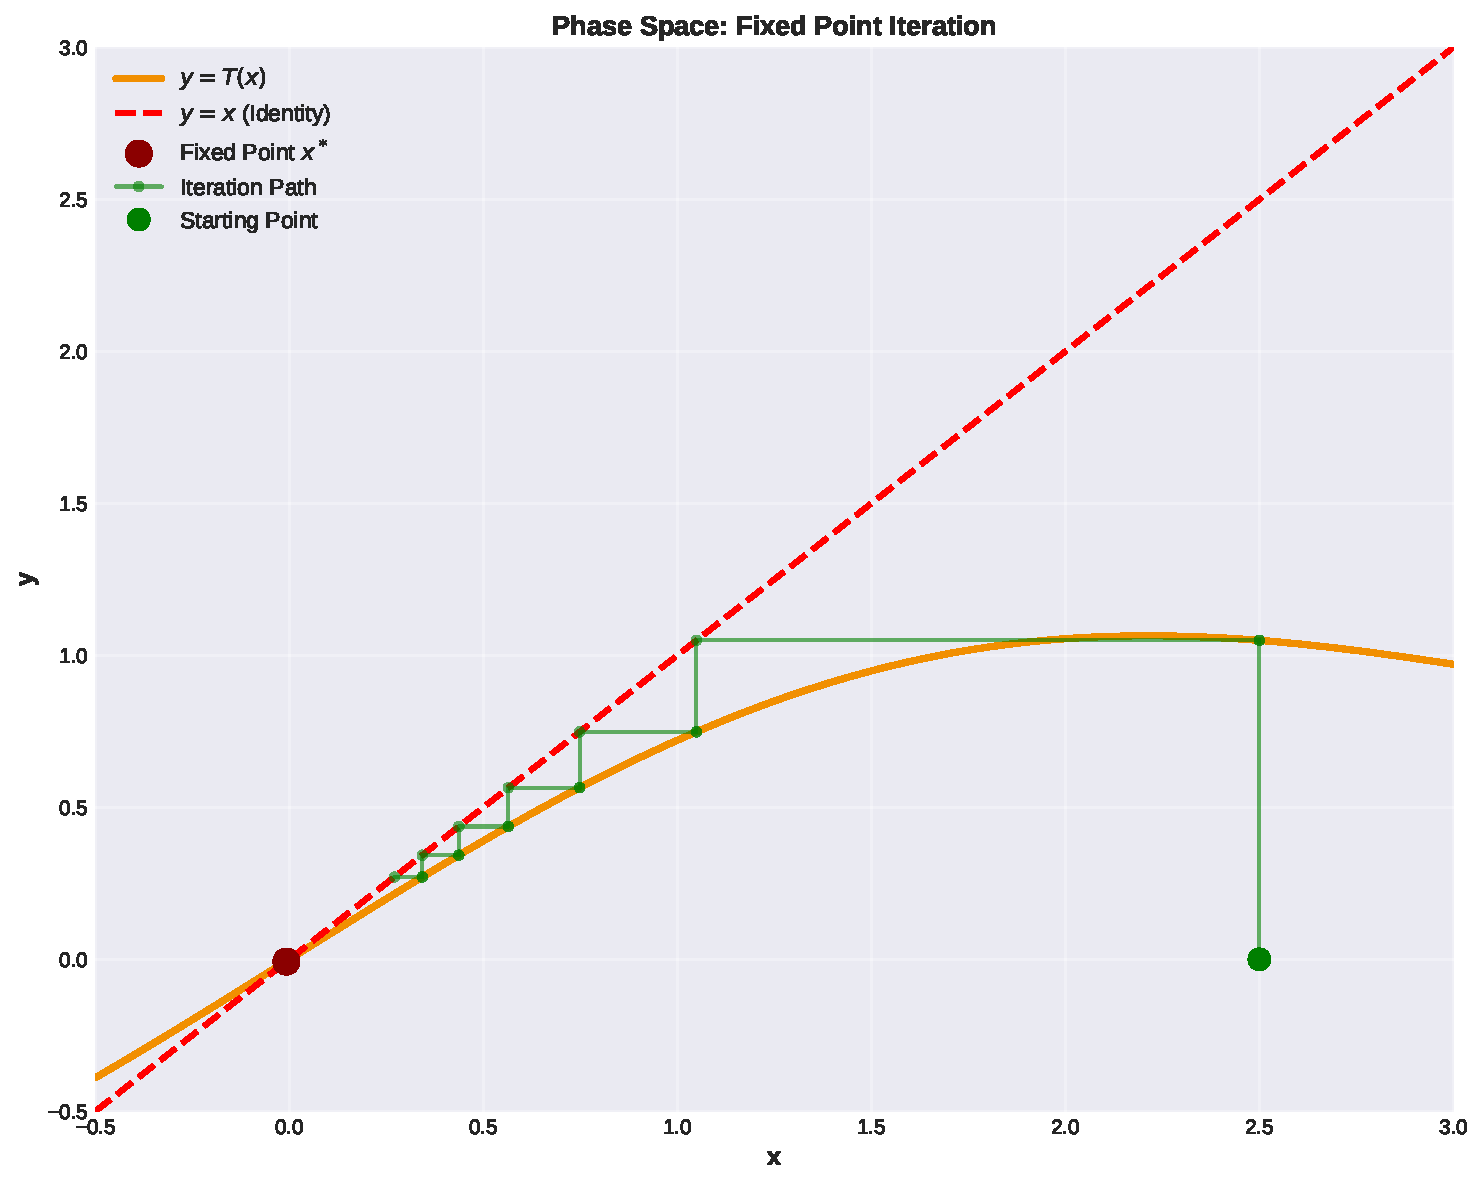
\includegraphics[width=0.9\linewidth]{phase_space}
\end{center}

\textbf{Graphical Iteration Method:}
\begin{enumerate}
  \item Plot $y = T(x)$ and $y = x$ (identity line)
  \item Fixed points are intersections
  \item Follow the cobweb pattern to visualize convergence
  \item Distance to fixed point decreases with proper choice of parameters
\end{enumerate}

\end{frame}

% ============================================================================
% SECTION 6: ADVANCED TOPICS
% ============================================================================

\section{Advanced Topics}

\begin{frame}{Convergence Under Weak Contractions}

\begin{definition}[Weak Contraction]
A mapping $T: X \to X$ is called a \textbf{weak contraction} if:
$$\|T(x) - T(y)\| < \|x - y\| \quad \text{for all } x \neq y$$
without requiring a fixed Lipschitz constant.
\end{definition}

\vspace{0.3cm}

\begin{theorem}[Edelstein's Theorem]
If $T$ is a weak contraction on a complete metric space $X$, and the orbit $\{T^n(x_0)\}$ has a convergent subsequence, then the limit point is a unique fixed point of $T$ in a neighborhood of $x_0$.
\end{theorem}

\vspace{0.3cm}

\textbf{Application to Noor:} Noor iteration converges even when $T$ is only a weak contraction, provided parameter sequences satisfy convergence conditions.

\end{frame}

\begin{frame}{Nonexpansive Mappings}

\begin{definition}[Nonexpansive Mapping]
A mapping $T: C \to C$ is \textbf{nonexpansive} if:
$$\|T(x) - T(y)\| \leq \|x - y\| \quad \forall x, y \in C$$
\end{definition}

\vspace{0.3cm}

\begin{block}{Comparison with Contractions}
\begin{itemize}
  \item Nonexpansive maps need not have fixed points (unlike contractions)
  \item Require additional conditions: $C$ compact or convex
  \item Multiple fixed points are possible
  \item Noor iteration handles nonexpansive mappings with appropriate modifications
\end{itemize}
\end{block}

\vspace{0.3cm}

\begin{theorem}
For nonexpansive mappings on compact convex sets in Hilbert spaces, Noor iteration with appropriate parameter sequences converges weakly to a fixed point.
\end{theorem}

\end{frame}

\begin{frame}{Weak Convergence vs Strong Convergence}

\begin{definition}[Strong Convergence]
A sequence $\{x_n\}$ in a Banach space $X$ is \textbf{strongly convergent} to $x^* \in X$ if:
$$\lim_{n \to \infty} \|x_n - x^*\| = 0$$
\end{definition}

\vspace{0.3cm}

\begin{definition}[Weak Convergence]
A sequence $\{x_n\}$ in $X$ is \textbf{weakly convergent} to $x^* \in X$ if:
$$\lim_{n \to \infty} \langle f(x_n) \rangle = \langle f(x^*) \rangle \quad \text{for all } f \in X^*$$
\end{definition}

\vspace{0.3cm}

\textbf{For Noor Iteration:}
\begin{itemize}
  \item Guarantees \textbf{strong convergence} for contractions
  \item Achieves \textbf{weak convergence} for nonexpansive mappings in certain spaces
  \item Choice of Banach space structure affects convergence type
\end{itemize}

\end{frame}

\begin{frame}{Stability and Perturbation Analysis}

\begin{block}{Stability Question}
If $T$ is slightly perturbed to $T_\epsilon = T + \epsilon F$, do the fixed points vary continuously?
\end{block}

\vspace{0.3cm}

\begin{theorem}[Implicit Function Theorem Application]
If $T$ is continuously Fréchet differentiable and $\mathbf{1} - DF(x^*)$ is invertible (where $x^*$ is the fixed point), then fixed points vary continuously with small perturbations.
\end{theorem}

\vspace{0.3cm}

\textbf{For Noor Iteration:}
\begin{itemize}
  \item Stability of the iteration depends on the spectral radius of $DF(x^*)$
  \item Smaller step sizes ($a_n, b_n, c_n$) increase stability
  \item Robustness to rounding errors increases with smaller parameters
\end{itemize}

\end{frame}

% ============================================================================
% SECTION 7: APPLICATIONS TO PDEs AND INTEGRAL EQUATIONS
% ============================================================================

\section{Applications}

\begin{frame}{Application 1: Differential Equations}

\begin{example}[Two-Point Boundary Value Problem]
Consider the boundary value problem:
\begin{align*}
-x''(t) + h(t)x(t) &= f(t), \quad t \in (0,1)\\
x(0) &= x(1) = 0
\end{align*}

This can be rewritten as a fixed point problem: $x = Gx$ where
$$G(x)(t) = \int_0^1 G_0(t,s)[f(s) + h(s)x(s)] ds$$
with $G_0$ the Green's function.
\end{example}

\vspace{0.2cm}

\textbf{Solution Strategy:}
\begin{enumerate}
  \item Show $G$ is a contraction (or weak contraction) on $C[0,1]$
  \item Apply Noor iteration to compute the solution
  \item Use parameter sequences to ensure rapid convergence
\end{enumerate}

\end{frame}

\begin{frame}{Application 2: Integral Equations}

\begin{example}[Volterra Integral Equation]
The second-kind Volterra equation:
$$x(t) = f(t) + \int_0^t K(t,s,x(s)) ds$$

defines a fixed point problem where $T(x)(t) = f(t) + \int_0^t K(t,s,x(s)) ds$.
\end{example}

\vspace{0.3cm}

\textbf{Analysis:}
\begin{itemize}
  \item Contractivity depends on kernel $K$ and bounds
  \item Noor iteration provides numerical solution with error control
  \item Parameter sequences optimize computational efficiency
  \item Applications: heat equations, diffusion, kinetic equations
\end{itemize}

\vspace{0.3cm}

\begin{theorem}[Convergence for Volterra Equations]
If $|K(t,s,x_1) - K(t,s,x_2)| \leq L|x_1 - x_2|$ with small enough Lipschitz constant $L$, Noor iteration converges to the unique solution.
\end{theorem}

\end{frame}

\begin{frame}{Application 3: Optimization Problems}

\begin{block}{Minimization via Fixed Points}
Optimization problems can be converted to fixed point problems:
$$\min_{x \in \mathcal{C}} f(x) \quad \Rightarrow \quad x = P_\mathcal{C}(\nabla f(x))$$
where $P_\mathcal{C}$ is the projection onto the convex set $\mathcal{C}$.
\end{block}

\vspace{0.3cm}

\begin{itemize}
  \item Gradient descent is a special case of iteration
  \item Proximal methods use fixed points of proximal operators
  \item Noor iteration can accelerate convergence in optimization
  \item Important in machine learning and signal processing
\end{itemize}

\vspace{0.3cm}

\begin{example}
Proximal gradient algorithm for minimizing $f(x) + g(x)$:
$$x_{n+1} = \text{prox}_{g}(x_n - \nabla f(x_n))$$
is a fixed point iteration where $T = \text{prox}_g \circ (I - \nabla f)$.
\end{example}

\end{frame}

% ============================================================================
% SECTION 8: SUMMARY AND CONCLUSION
% ============================================================================

\section{Summary and Conclusion}

\begin{frame}{Key Takeaways}

\begin{enumerate}
  \item \textbf{Noor Iteration} is a three-step fixed point iteration method that generalizes Mann and Ishikawa iterations

  \vspace{0.2cm}

  \item \textbf{Convergence} is guaranteed under:
  \begin{itemize}
    \item Contractive mappings (or weak contractions)
    \item Appropriate parameter sequences satisfying theoretical conditions
    \item Proper choice of Banach space structure
  \end{itemize}

  \vspace{0.2cm}

  \item \textbf{Fixed Point Theorems} (Banach, Krasnoselski, etc.) provide the theoretical foundation for guaranteeing existence and uniqueness of fixed points

  \vspace{0.2cm}

  \item \textbf{Applications} span differential equations, integral equations, optimization, and numerical analysis

  \vspace{0.2cm}

  \item \textbf{Practical Implementation} requires careful parameter selection to balance convergence speed with computational cost

\end{enumerate}

\end{frame}

\begin{frame}{Further Reading}

\begin{thebibliography}{10}

  \bibitem{Pathak2018}
  Pathak, H.K. (2018)
  \textit{An Introduction to Nonlinear Analysis and Fixed Point Theory}
  Springer

  \bibitem{Kirk2001}
  Kirk, W.A. (2001)
  Fixed point theorems in nonempty compact convex sets
  \textit{In: Handbook of Metric Fixed Point Theory}

  \bibitem{Browder1965}
  Browder, F.E. (1965)
  Nonexpansive nonlinear operators in Banach spaces
  \textit{Proceedings of the National Academy of Sciences}

  \bibitem{Mann1953}
  Mann, W.R. (1953)
  Mean value methods in iteration
  \textit{Proceedings of the American Mathematical Society}, 4(3), 506-510

  \bibitem{Ishikawa1974}
  Ishikawa, S. (1974)
  Fixed points and iteration of commuting nonexpansive mappings
  \textit{Pacific Journal of Mathematics}

\end{thebibliography}

\end{frame}

\begin{frame}{Conclusion}

\begin{block}{Significance of Noor Iteration}
Noor iteration represents a sophisticated yet practical approach to finding fixed points in nonlinear functional analysis. It combines:
\begin{itemize}
  \item Mathematical rigor through fixed point theorems
  \item Computational efficiency through multi-step schemes
  \item Practical applicability to real-world problems
\end{itemize}
\end{block}

\vspace{0.4cm}

\begin{block}{Future Directions}
\begin{itemize}
  \item Acceleration techniques (Anderson, Nesterov-type)
  \item Parallel and distributed implementations
  \item Applications to machine learning and deep learning
  \item Variable order step methods
\end{itemize}
\end{block}

\vspace{0.4cm}

\textbf{The study of fixed point iterations continues to be central to numerical analysis and optimization.}

\end{frame}

\end{document}
